%----------------------------------------------------------------------------------------
%	PACKAGES AND OTHER DOCUMENT CONFIGURATIONS
%----------------------------------------------------------------------------------------

\documentclass[11pt,a4paper]{article}
\usepackage[english]{babel}
\usepackage[utf8x]{inputenc}
\usepackage{amsmath}
\usepackage{graphicx}
\usepackage[colorinlistoftodos]{todonotes}
\usepackage{gensymb}
\usepackage{geometry}
 \geometry{a4paper, total={160mm,247mm}, left=25mm, top=25mm}
\usepackage{wrapfig}
\usepackage{float}
\usepackage{listings} %code
\usepackage{pagecolor} %black title page
\usepackage{aurical} %title page font
\usepackage[T1]{fontenc} %title page font
\usepackage{lipsum} %fillers
\usepackage{epigraph} %quotations
% Rotate table  headers
\usepackage{adjustbox}
\usepackage{array}
\newcolumntype{R}[2]{%
    >{\adjustbox{angle=#1,lap=\width-(#2)}\bgroup}%
    l%
    <{\egroup}%
}
\newcommand*\rot{\multicolumn{1}{R{45}{1em}}}% no optional argument here, please!

\setlength{\parindent}{0pt}
\setlength{\parskip}{1em}

\begin{document}

\newcommand\numberthis{\addtocounter{equation}{1}\tag{\theequation}}

\begin{titlepage}
\pagecolor{black!90}
\color{red}
\Fontskrivan
\newcommand{\HRule}{\rule{\linewidth}{0.5mm}} % Defines a new command for the horizontal lines, change thickness here


\center % Center everything on the page
 
%----------------------------------------------------------------------------------------
%	HEADING SECTIONS
%----------------------------------------------------------------------------------------

\textsc{\LARGE Linköpings Universitet}\\[0.5cm] % Name of your university/college
\textsc{\Large 732A92 - Textmining}\\[0.5cm] % Major heading such as course name
\textsc{\large }\\[4.5cm] % Minor heading such as course title

%----------------------------------------------------------------------------------------
%	TITLE SECTION
%----------------------------------------------------------------------------------------

\HRule \\[0.4cm]
{ \huge \bfseries Are horror movies really what they claim?}\\[0.4cm] % Title of your document
\HRule \\[1.5cm]
 
%----------------------------------------------------------------------------------------
%	AUTHOR SECTION
%----------------------------------------------------------------------------------------

\begin{minipage}{0.4\textwidth}
\begin{flushleft} \large
\emph{Author:}\\
Gustav \textsc{Lundberg} \\ % Your name 
guslu389
\end{flushleft}
\end{minipage}
~
\begin{minipage}{0.4\textwidth}
\begin{flushright} \large
\emph{Examiner:} \\
Marco \textsc{Kuhlmann} % Supervisor's Name
\end{flushright}
\end{minipage}\\[2cm]
%----------------------------------------------------------------------------------------
%	DATE SECTION
%----------------------------------------------------------------------------------------

{\large \today}\\[2cm] % Date, change the \today to a set date if you want to be precise

%----------------------------------------------------------------------------------------
%	LOGO SECTION
%----------------------------------------------------------------------------------------
\vfill % Fill the rest of the page with whitespace

\includegraphics[width=60mm]{LiU_logo.PNG} % Include a department/university logo - this will require the graphicx package

%----------------------------------------------------------------------------------------
\end{titlepage}

\pagecolor{none}
\color{black}
%----------------------------------------------------------------------------------------
%	ASTRACT
%----------------------------------------------------------------------------------------
\pagenumbering{gobble}
\begin{abstract}
    \lipsum[83-84]
\end{abstract}
\newpage

%----------------------------------------------------------------------------------------
%	INNEHÅLLSFÖRTECKNING
%----------------------------------------------------------------------------------------
\tableofcontents

\newpage

%----------------------------------------------------------------------------------------
%	HUVUDTEXT
%----------------------------------------------------------------------------------------
\pagenumbering{arabic}
\renewcommand\thetable{\thesection.\arabic{table}}
\renewcommand\thefigure{\thesection.\arabic{figure}}    
\setcounter{figure}{0}  

\section{Introduction}

\epigraph{My experience of life is that it is not divided up into genres; it’s a horrifying, romantic, tragic, comical, science-fiction cowboy detective novel. You know, with a bit of pornography if you're lucky.}{\textit{Alan Moore}}

In the world of movies, a genre is a label that gives the viewer a rough sense on what to expect from the movie. A \textit{Sci-fi}-movie will likely have elements of technology that are not feasible today (or at the time of production at least), a \textit{romantic} movie will have a good portion of love and an \textit{action} movie shouldn't lead to you falling asleep. A movie can of course contain elements from multiple genres; a \textit{romantic comedy} is expected to contain love and laughter while an \textit{adventure-sports-musical} will likely be just weird... 

The genres do however only represent a rough outline of the movie (or artistic work of any kind really), and thus the movie may contain generic elements of various kinds (affection, fear, joy, camaraderie, historical depictions etc) while only being considered to belong in a single genre. The genres can further be divided into sub-genres.

From a statistical or machine-learning perspective, movies are interesting since they are definitely a form of categories, but an observation or sample (movie, book painting etc) can be flagged with multiple genres. As mentioned above, the works will likely contain elements from further genres but not to an extent that the entire work can be considered a member of those genres as well. There is no maximum number of categories an observation can be part of and the genres themselves are binary (either the movie is a comedy or not) while the amount of corresponding content represent a continuous  variable we can end up in interesting problems. 

The problem this project sets out to solve is whether you can derive the different genres a movie is part of by just looking at the synopsis of the movie. More specifically, we delve into the world of horror movies since these commonly mix a few general concepts only and those are at least somewhat distinct. Such concepts may include zombies, ghosts, monsters, murderers and more, but you don't often try to mix as many of them as possible into a single movie. This is done by applying topic modelling to the movie descriptions and analysing the result. The title will also be included in the topic model to see whether this affects the topics in any way, the thought being that movies may be named in somewhatsimilar ways but described differently.

The project at the same time tries to see whether the additional genres some horror movies are flagged with can be derived from the same synopses. This is done in part by applying a density based clustering algorithm to the movie descriptions and in part by analysing the topic modelling previously mentioned. The choice to use density based clustering in done since far from every movie has an additional genre attached to it and it is thus necessary to be able to consider some movies as outside of any clusters.

\newpage


\section{Data and feature construction}

The data set comes from Kaggle via PromptCloudHQ that has scraped IMDB for all movies tagged with the horror genre released between 2012 and 2017, a total of 3328 entries. Included in the data are 12 variables such as the title of the movie, a pipe-separated list of genres and a short summary of the plot of the movie as well as release date, run time and reviewer rating. In this project, the first three of these are used.

\subsection{Title field}

The title field of course contains the name of the movie, but also the year of release within parenthesis. For examples see table \ref{tab:title_examples}. The release year information was removed using R and some regular expressions via the \verb|stringr|-package.


\begin{table}[ht]
\centering
\label{tab:title_examples}
\begin{tabular}{ll}
  \hline
 \textbf{Before cleaning} & \textbf{After cleaning} \\ 
  \hline
 V/H/S/2 (2013) & V/H/S/2 \\ 
 Chudail Story (2016) & Chudail Story \\ 
 Bigfoot vs. D.B. Cooper (2014) & Bigfoot vs. D.B. Cooper \\ 
   \hline
\end{tabular}
\caption{Examples of movie titles before and after removal of release year}
\end{table}

\subsection{List of genres}

In order to compare the clusters of movies and the genres they have been flagged with, it is easier to have a binary matrix indicating whether or not a movie was flagged with the particular genre than a list of genres. This is done by splitting the list at each pipe and checking what genres are found in the split list by comparing to a list of all genres. For examples see table \ref{tab:genre_examples}

\begin{table}[t]
\centering
\label{tab:genre_examples}
\begin{tabular}{lrrrrrrrrrr}
  \hline
\textbf{Genre list} & \rot{Action} & \rot{Adventure} & \rot{Comedy} & \rot{Crime} & \rot{Drama} & \rot{Fantasy} & \rot{Mystery} & \rot{Romance} & \rot{Sci-Fi} & \rot{Thriller} \\ 
  \hline
Horror & 0 &   0 &   0 &   0 &   0 &   0 &   0 &   0 &   0 &   0 \\ 
Drama$|$ Horror$|$ Mystery$|$ Thriller &  0 & 0 &   0 &   0 &   1 &   0 &   1 &   0 &   0 &   1 \\ 
Action$|$ Horror$|$ Sci-Fi & 0 &  0 &   0 &   0 &   0 &   0 &   0 &   0 &   1 &   0 \\
   \hline
\end{tabular}
\caption{Examples of genres representation before and after cleaning}
\end{table}

At this stage, a bit of filtering was done as some genres are found in only a small number of films. A minimum of 90 movies were required for the genre to be included. Since All movies were flagged as horror movies, this genre is not included either. This resulted in a total of ten out of the original 22 genres being included. For an overview of the number of movies by genre, see figure \ref{fig:genre_dist}.

\begin{figure}[ht]
\label{fig:genre_dist}
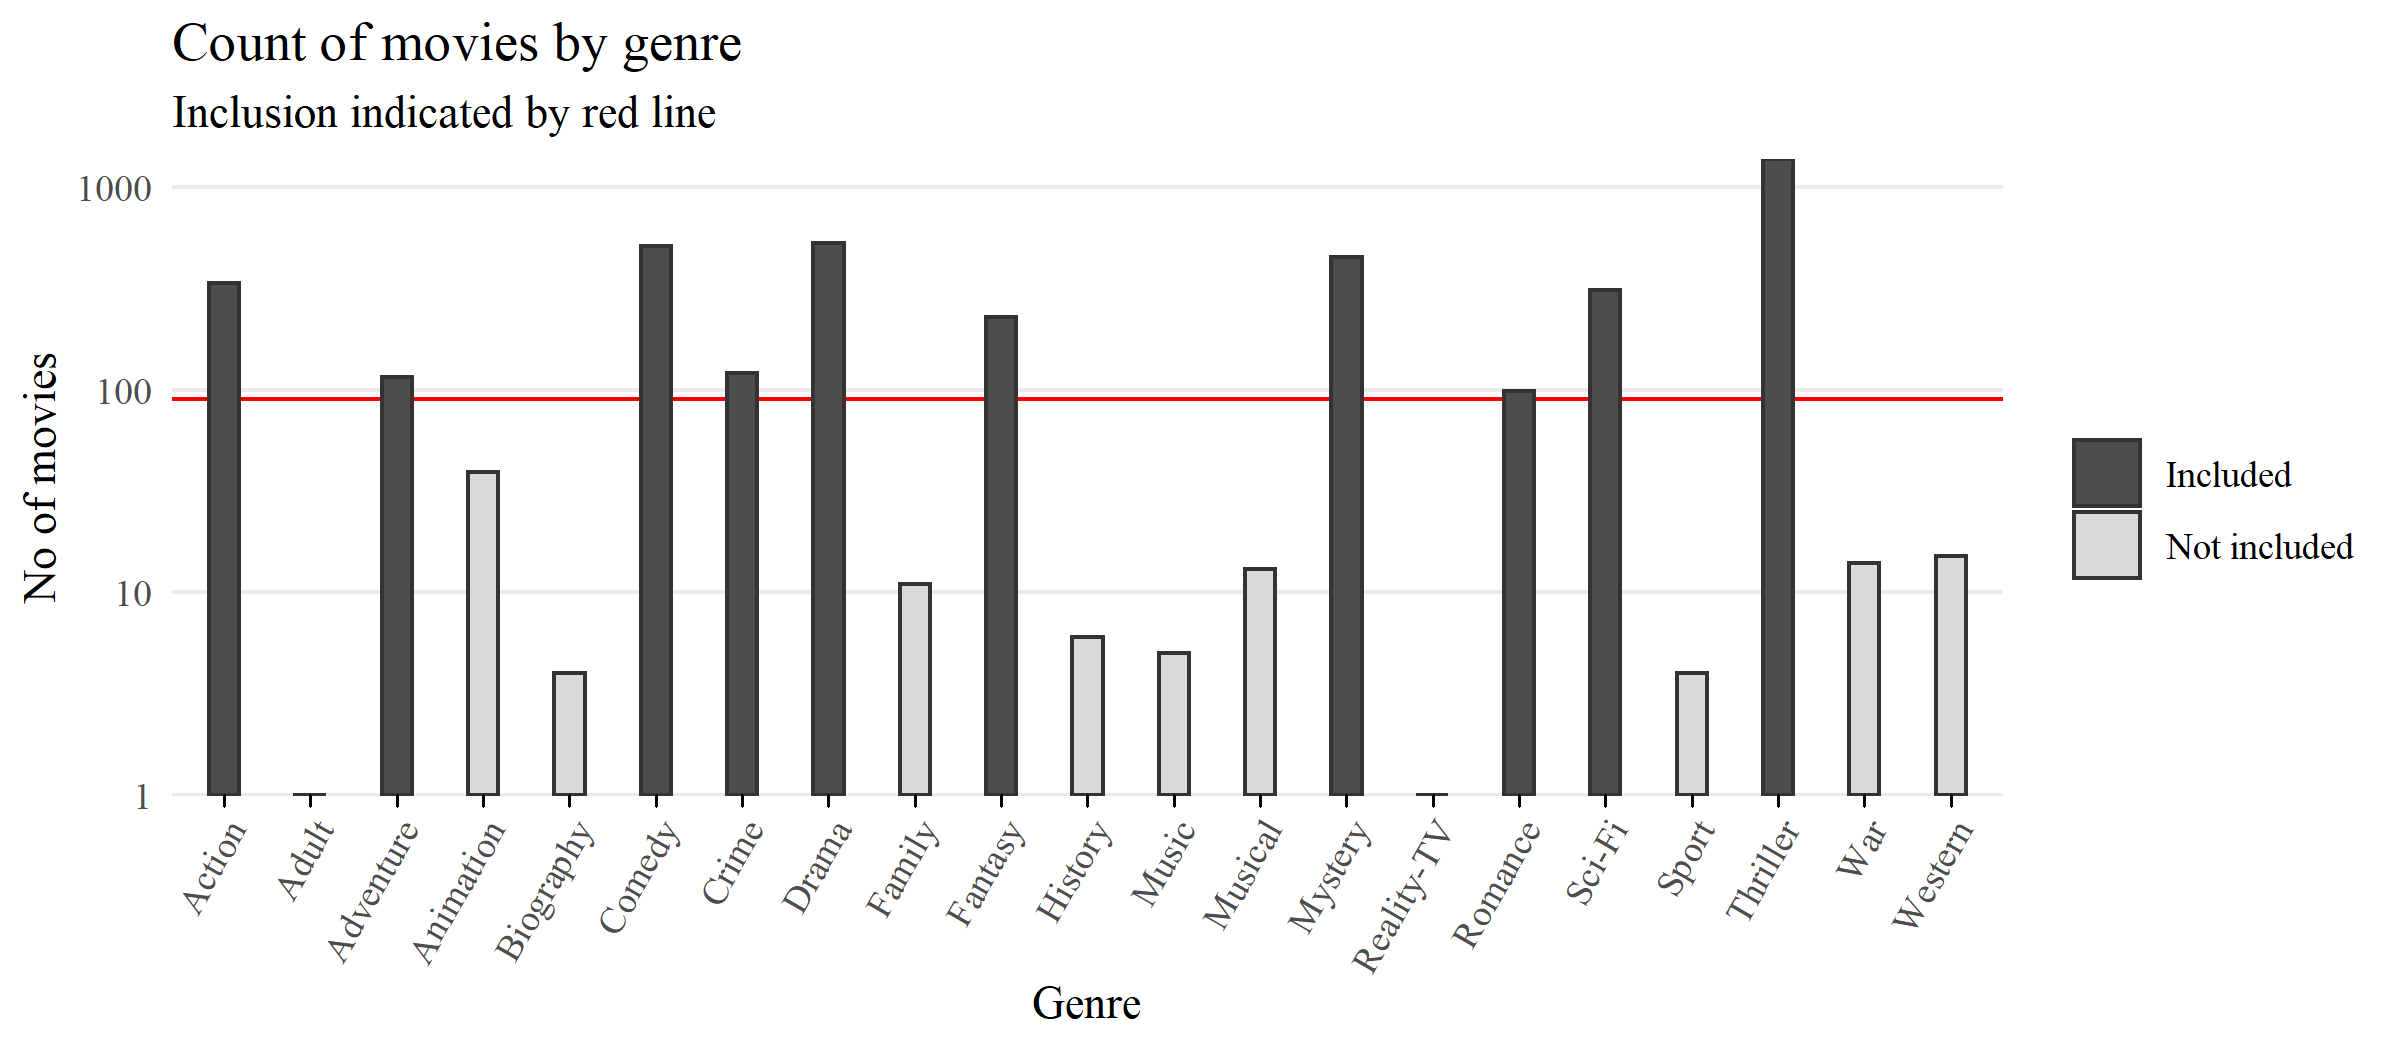
\includegraphics[width=1.1 \textwidth]{genre_dist.png}
\caption{Count of movies by genre}
\centering
\end{figure}

\subsection{Plot field}

The movie plots are the main data source for the project, and also the field that required the most work to get to a usable format. In the raw data, the plot field also contain information about the director and the cast in the movie, in most cases at least. The names of the cast and director contain all sorts of special characters that needed to be removed by way of regular expressions. For examples of before and after cleaning of the field, see table \ref{tab:plot_examples}.

Before being used in the clustering and topic modelling, the plot fields also go trough lemmatization, stop word removal, and lower casing. Finally, they are run through the tfidf-vectorizer and combined with the title field creating a tfidf-representation of the plot with and without the title for comparison.

\begin{table}[ht]
\centering
\label{fig:plot_examples}
\begin{tabular}{p{8cm}p{8cm}}
  \hline
 \textbf{Before cleaning} & \textbf{After cleaning} \\ 
  \hline
 Directed by Piotr Matwiejczyk. With Dawid Antkowiak, Justyna Boczulak, Marcin Bosak, Milosz Bugajski. &  \\ 
 \hline
 Directed by John Beaton Hill. With David Cooley, Brian Scannell, Kurt Fuller, Jack McGee. Childhood friends from Boston drift apart following a shocking discovery deep in the woods of Savin Hill. Years later a tragic murder brings them together again. But for one man, its no mistake. A trap has been set... After serving time for a crime he didnt commit, TOM GREYS is released from prison with a score to settle: he is deadset on tracking down the man who set him up... his childhood ... & Childhood friends from Boston drift apart following a shocking discovery deep in the woods of Savin Hill. Years later a tragic murder brings them together again. But for one man, its no mistake. A trap has been set... After serving time for a crime he didnt commit, TOM GREYS is released from prison with a score to settle: he is deadset on tracking down the man who set him up... his childhood ... \\ 
 \hline
 Directed by Adrián García Bogliano, Ramiro García Bogliano. With Cristina Brondo, Camila Bordonaba, Berta Muñiz, Arnaldo André. A woman hesitantly rents an apartment to an eerie man who she soon realizes has a part in the solar eclipse that is taking place. & A woman hesitantly rents an apartment to an eerie man who she soon realizes has a part in the solar eclipse that is taking place. \\ 
   \hline
\end{tabular}
\caption{Examples of plots before and after cleaning}
\end{table}

\clearpage

\section{Method}

\subsection{Topic Modelling}

As mentioned; topic modelling will be used to try an find the subgenres of the movies. Since this method was used in the course, it will not be presented here as well.

\subsection{Clustering using DBSCAN}

The clustering method used in the course, k-means, has a great drawback in that it cannot leave points unclustered. Since a lot of the movies will only be considered horror movies and not be part of another genre, a method that can consider observations as outside clusters is needed. 

One such method is DBSCAN, a density based clustering algorithm first proposed in 1996. 


\newpage


\section{Result}

\lipsum[21-25]

\newpage

\section{Discussion}

\lipsum[25-30]

\newpage

\section{Conclusion}

\lipsum[30-35]

\newpage

\end{document}